\documentclass[twoside]{article}
\usepackage{aistats2016}
\usepackage{hyperref}
\usepackage{amsmath, amssymb, amsthm, graphicx, algorithm}
\usepackage{algpseudocode}
\usepackage{caption}
\usepackage{subcaption}
\usepackage{blkarray}
\usepackage{xcolor}
\usepackage[all,cmtip]{xy}

% If your paper is accepted, change the options for the package
% aistats2016 as follows:
%
%\usepackage[accepted]{aistats2016}
%
% This option will print headings for the title of your paper and
% headings for the authors names, plus a copyright note at the end of
% the first column of the first page.

\newcommand{\A}{\mathcal{A}}
\newcommand{\C}{\mathcal{C}}
\newcommand{\D}{\mathcal{D}}
\newcommand{\G}{\mathcal{G}}
\newcommand{\B}{\mathcal{B}}
\newcommand{\E}{\mathcal{E}}
\newcommand{\cS}{\mathcal{S}}
\newcommand{\U}{\mathcal{U}}
\newcommand{\cL}{\mathcal{L}}
\newcommand{\N}{\mathcal{N}}
\newcommand{\cO}{\mathcal{O}}
\newcommand{\M}{\mathcal{M}}
\newcommand{\bN}{\mathbb{N}}
\newcommand{\bQ}{\mathbb{Q}}
\newcommand{\Exp}{\mathbb{E}}
\newcommand{\bC}{\mathbb{C}}
\newcommand{\bR}{\mathbb{R}}
\newcommand{\bZ}{\mathbb{Z}}
\newcommand{\bK}{\mathbb{K}}
\newcommand{\bF}{\mathbb{F}}

\newcommand{\fF}{\mathbf{F}}
\newcommand{\fA}{\mathbf{A}}
\newcommand{\Grp}{\mathbf{Grp}}
\newcommand{\Set}{\mathbf{Set}}
\newcommand{\Mor}{\mathrm{Mor}}
\newcommand{\Aut}{\mathrm{Aut}}
\newcommand{\Gal}{\mathrm{Gal}}
\newcommand{\Char}{\mathrm{char}}
\newcommand{\SL}{\mathrm{SL}}
\newcommand{\GL}{\mathrm{GL}}
\newcommand{\Span}{\mathrm{span}}
\newcommand{\Hom}{\mathrm{Hom}}
\newcommand{\Ext}{\mathrm{Ext}}
\newcommand{\im}{\mathrm{im}}
\newcommand{\col}{\mathrm{col}}
\newcommand{\argmax}{\mathrm{argmax}}
\newcommand{\cone}{\mathrm{cone}}
\newcommand{\rank}{\mathrm{rank}}
\newcommand{\RP}{\mathbb{R}\mathrm{P}}
\newcommand{\tr}{\mathrm{tr}}

\newcommand{\df}{\overset{\text{def}}{=}}
%\newcommand{\deg}{\mathrm{deg}}

\newcommand{\vx}{\mathbf{x}}
\newcommand{\vy}{\mathbf{y}}
\newcommand{\vu}{\mathbf{u}}
\newcommand{\vv}{\mathbf{v}}
\newcommand{\va}{\mathbf{a}}
\newcommand{\vb}{\mathbf{b}}
\newcommand{\vc}{\mathbf{c}}
\newcommand{\vd}{\mathbf{d}}
\newcommand{\vg}{\mathbf{g}}
\newcommand{\vk}{\mathbf{k}}
\newcommand{\vw}{\mathbf{w}}
\newcommand{\vz}{\mathbf{z}}
\newcommand{\vp}{\mathbf{p}}
\newcommand{\vq}{\mathbf{q}}
\newcommand{\vS}{\mathbf{S}}
\newcommand{\vf}{\mathbf{f}}
\newcommand{\bo}{\mathbf{1}}
\newcommand{\bz}{\mathbf{0}}
\newcommand{\id}{\mathrm{id}}

\theoremstyle{theorem}
\newtheorem{thm}{Theorem}

\theoremstyle{theorem}
\newtheorem{prop}{Proposition}
\theoremstyle{theorem}
\newtheorem{cor}{Corollary}

\theoremstyle{lemma}
\newtheorem{lemma}{Lemma}

\theoremstyle{definition}
\newtheorem{defn}{Definition}

\theoremstyle{example}
\newtheorem{ex}{Example}

\newcommand\undermat[2]{%
  \makebox[0pt][l]{$\smash{\underbrace{\phantom{%
    \begin{matrix}#2\end{matrix}}}_{\text{$#1$}}}$}#2}
    
\newcommand\overmat[2]{%
  \makebox[0pt][l]{$\smash{\color{black}\overbrace{\phantom{%
    \begin{matrix}#2\end{matrix}}}^{\text{\color{black}#1}}}$}#2}


\begin{document}
\input xy
\xyoption{all}
\xyoption{arc}
\makeatletter
\def\BState{\State\hskip-\ALG@thistlm}
\makeatother
% If your paper is accepted and the title of your paper is very long,
% the style will print as headings an error message. Use the following
% command to supply a shorter title of your paper so that it can be
% used as headings.
%
%\runningtitle{I use this title instead because the last one was very long}

% If your paper is accepted and the number of authors is large, the
% style will print as headings an error message. Use the following
% command to supply a shorter version of the authors names so that
% they can be used as headings (for example, use only the surnames)
%
%\runningauthor{Surname 1, Surname 2, Surname 3, ...., Surname n}

\twocolumn[

\aistatstitle{Bayesian Models for Service Quality Analysis of the Boston City 311}

\aistatsauthor{ Jane Huang \And Isadora Nun \And Weiwei Pan \And Francisco Rivera}

\aistatsaddress{ Harvard University \And Harvard University \And Harvard University \And Harvard University} ]

\begin{abstract}
Fill in later.
\end{abstract}

\section{Introduction}

In 2015, Mayor Martin J. Walsh launched Boston 311, a platform to better enable residents of Boston to report non-emergency issues to the City, such as graffiti and broken street lights, and access City services. The program is similar to the 311 program that has been in place in New York City since 2003, and is aimed to streamline City services for Boston's residents. There is now a number of on-going and active data-analytics research projects based on the database of 311 service requests.

We suspect that analysis of response times will show complex patterns of heterogeneity. In particular, we are interested in the significance of the impact of  factors such as geography or neighborhood demographics. We will approach this in two ways:
\begin{enumerate}
\item We propose to model latent classes in respone time to service requests in the city of Boston. City officials describe service response time as roughlly depending on the type of request and the volume of requests.  
\item We will model the service response time as a function of the type as well as the location of the request.
\end{enumerate}

\section{Background}
\subsection{Bayesian Gaussian Mixture Models}
We will assume that our data is given by $Y = (\vx_1,\dots , \vx_N )$, where $\vx_n\in \bR^M$ is a vector encoding the reported location of the problem (in terms of longitude and latitude) and the request type. We will assume that $Y$ has a pdf that is a mixture of $K$ number of Gaussian components with parameters $\mu = \{\mu_k :  1\leq k\leq K\}$ and $\Sigma = \{\Sigma_k :  1\leq k\leq K\}$. Let $\pi \in \bR^k$ denote the set of mixture coefficients for this model. Then, the likelihood of observing $y_i$, given $\theta, \pi$ is
\begin{align}
L(\vx_n) = p(\vx_n | \mu, \Sigma, \pi) = \sum_{k=1}^K\pi_k \N(\vx_n | \mu_k, \Sigma_k )
\end{align}
where $\pi_k$ is the mixture coefficient for the $k$-th component. 

Alternatively, we can model the component membership information as missing data. That is, we model the component membership indicators as a set of latent variables, $Z = (\vz_1, \ldots, \vz_N)$, where $\vz_n \in \bR^K$ is a binary vector encoding of the membership of the $n$-th data in the $k$-th component. That is,
\begin{align}
z_{nk} = \begin{cases}
1, & \vx_n\text{ belongs to the $k$-th component}\\
0, & \text{otherwise}
\end{cases}
\end{align}
We will assume that the probability of observing $\vz_n$, given the mixture coefficients, as
\begin{align}
p(\vz_n | \pi) = \prod_{k=1}^K \pi_k^{z_{nk}}.
\end{align}
Now, we can rewrite the likelihood of our data set $Y$ as
\begin{align}
L(Y) = \prod_{n=1}^N\prod_{k=1}^K \N(x_n| \mu_k, \Sigma^{-1}_k)^{z_{nk}}.
\end{align}
Finally, a basic generative model for our mixture can be specified by the following:
\begin{align}
\pi &\sim Dir(\alpha_0)\\
\Sigma^{-1}_k &\sim Wish(W_0, \nu_0)\\
\mu_k | \Sigma^{-1}_k &\sim \N(\eta_0, (\beta_0 \Sigma^{-1}_k )^{-1})\\
z_n | \pi &\sim \prod_{k=1}^K \pi_k^{z_{nk}}\\
x_n | Z, \mu, \Sigma^{-1} &\sim \prod_{k=1}^K \N(\mu_k, \Sigma^{-1}_k)^{z_{nk}}
\end{align}
Note that the parameters of our model is $\theta = (\alpha_0, W_0, \nu_0, \eta_0, \beta_0)$. 
\begin{center}
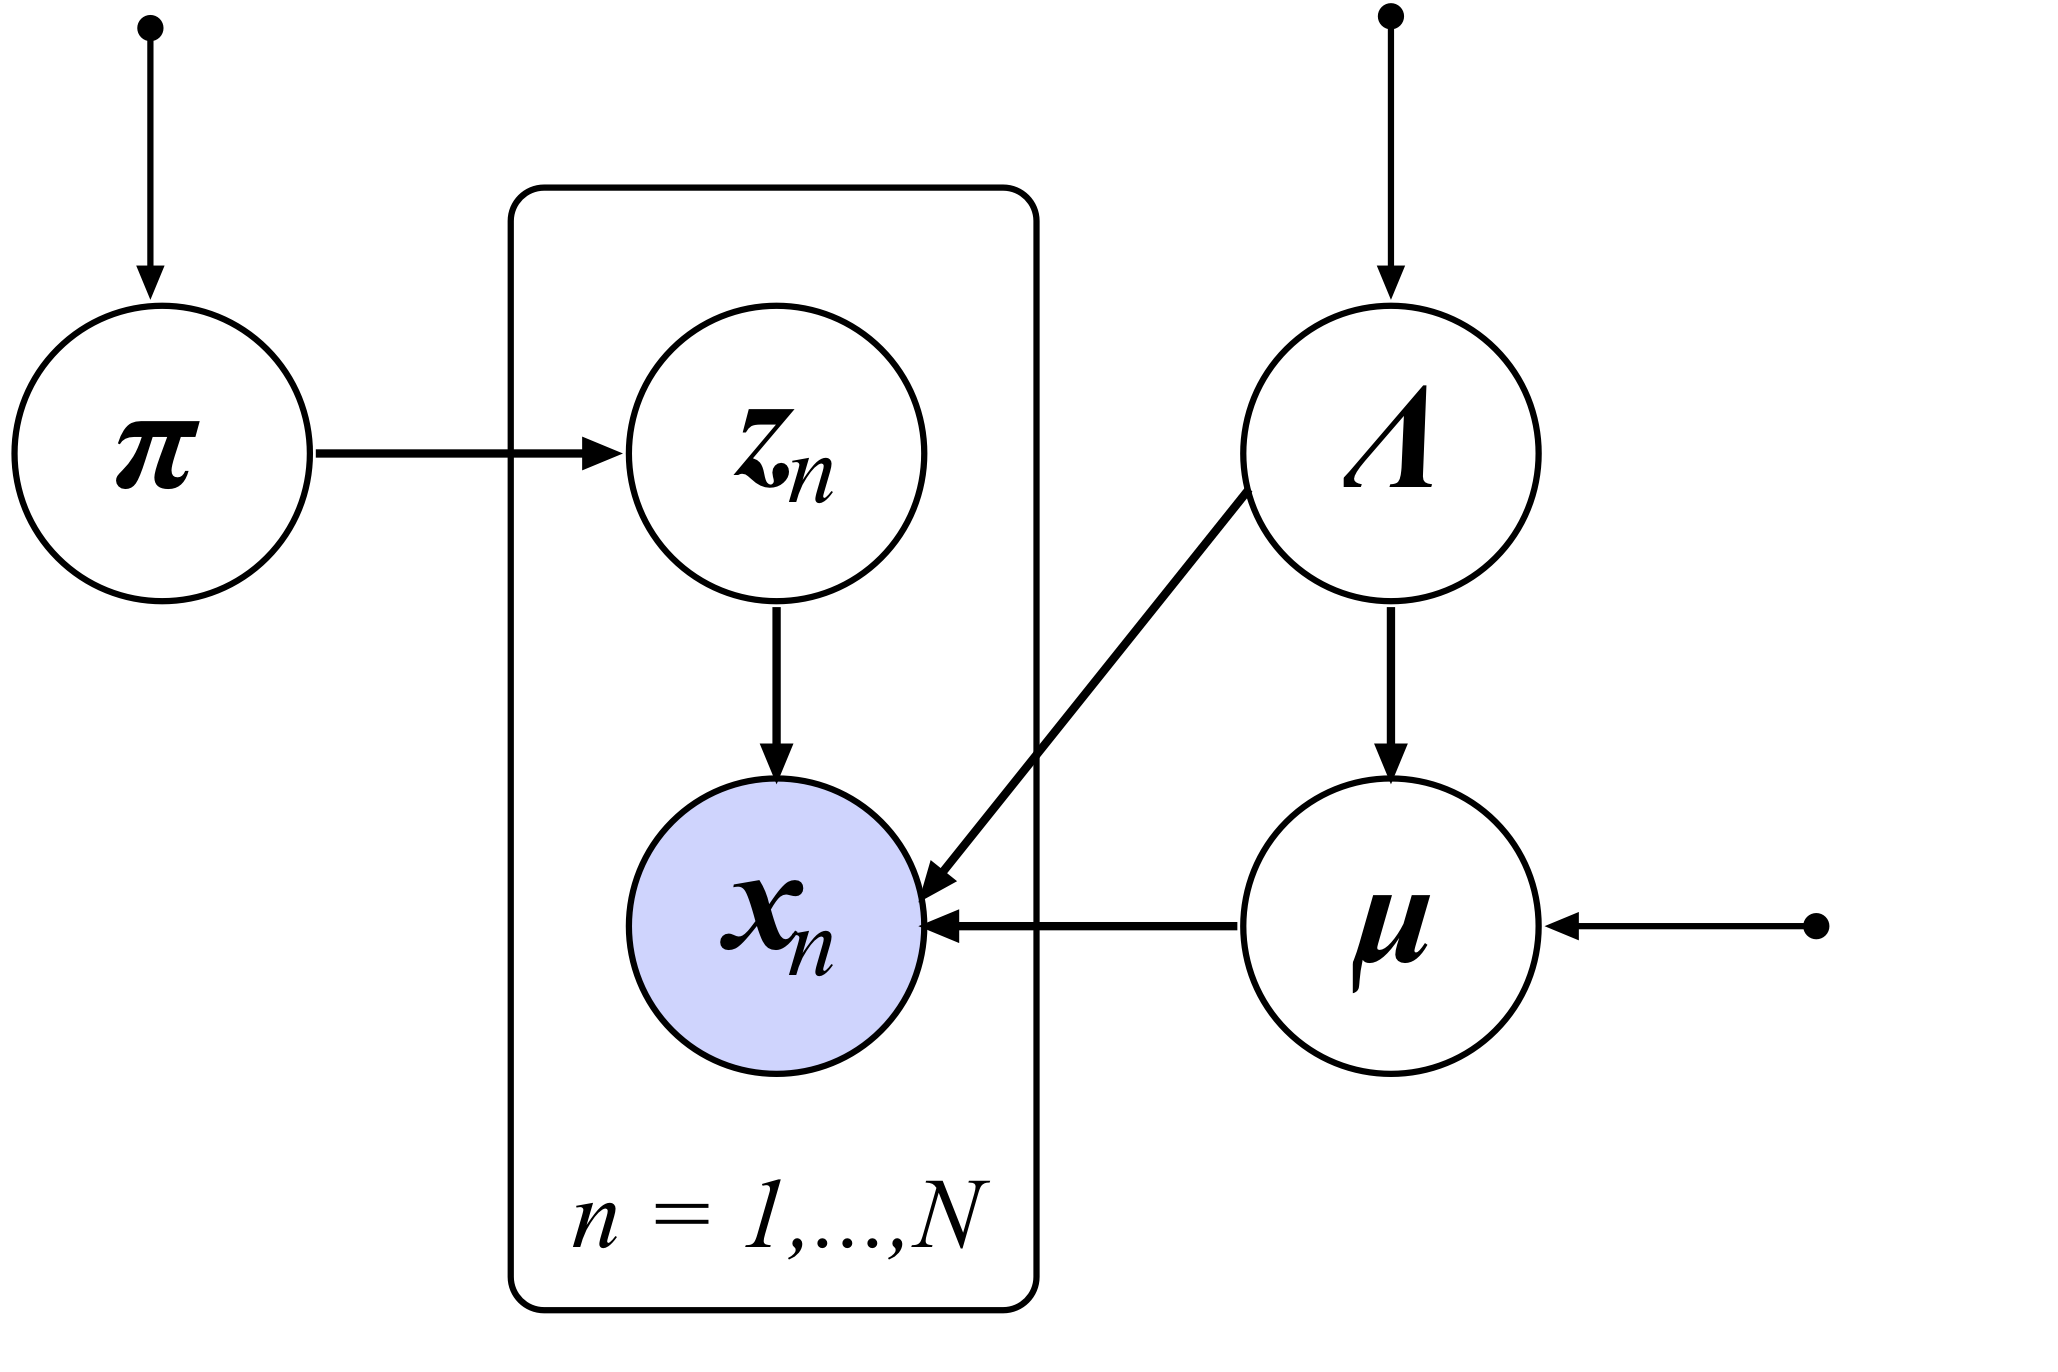
\includegraphics[width=50mm]{graph_model}
\end{center}

\subsection{Hamiltonian Monte Carlo within Gibbs Sampling}

\subsection{Variational Inference}

\section{Bayesian GMM with Demographic Information as Covariates}
\bibliographystyle{abbrv}
\bibliography{GMMBib}

\end{document}





